\documentclass[12pt, a4paper, twoside]{scrbook}
\usepackage{scrhack}
\usepackage[top=25mm, bottom=25mm, left=20mm, right=20mm]{geometry}

%\usepackage[utf8]{inputenc}
\usepackage[french]{babel}
\usepackage{csquotes}
\usepackage[unicode=true, breaklinks=true]{hyperref}
\usepackage[usenames,dvipsnames,hyperref,table]{xcolor}
\usepackage[format=plain, labelfont=bf]{caption}
\usepackage{subcaption}
\usepackage{enumitem}
\usepackage{transparent}

\usepackage{pgfplots}
\usepackage{makecell}
\usepackage{tikz}

\usepackage{setspace}
\usepackage{graphicx}
\usepackage{multicol}
\usepackage{tabularx}
\usepackage{makeidx}
\usepackage{wrapfig}
\usepackage{float}
\usepackage{framed}
\usepackage{siunitx}
\usepackage{transparent}
\usepackage[export]{adjustbox}

\usepackage{amsmath}
\usepackage{amssymb}
\usepackage{eqnarray}
\usepackage{breakcites}
\usepackage{fontawesome5}

\usepackage[pages=some]{background}
\usepackage{fancyhdr}
\pagestyle{fancy}

\def\pgf@lib@sh@rs@every@emptypart{}% clean slate
\special{pdf:minorversion 7}

\usetikzlibrary{
	shadows.blur,
	fit,
	arrows,
	arrows.meta,
	shapes,
	shapes.misc,
	shapes.arrows,
    shapes.geometric,
    shapes.multipart,
    patterns,
	chains,
	matrix,
	positioning,
	scopes,
	decorations.pathmorphing,
	shadows,
    calc,
    backgrounds,
}

%\addtolength{\tabcolsep}{-1pt}

\usepackage{pdfpages}
\usepackage{etoolbox}
\usepackage{titlesec}
%\usepackage {chapterbib}

%\usepackage{parskip}
\setlength{\partopsep}{-1em}
\setlength{\topsep}{-1em}
\setlength{\parsep}{-1em}
\setlength{\parskip}{1em}
\setlength{\parindent}{15pt}
\setlength{\itemsep}{-2em}
\setlength{\floatsep}{1em}
\setlength{\intextsep}{0em}
\setlength{\textfloatsep}{-1em}

% {left margin}{vspace before}{vspace after}
\titlespacing{\paragraph}{0em}{0em}{0em}
\titlespacing{\chapter}{0pt}{0em}{-2em}
\titlespacing{\section}{0pt}{0em}{0em}
\titlespacing{\subsection}{0pt}{0em}{0em}
\titlespacing{\subsubsection}{0pt}{0em}{-1em}


%\RedeclareSectionCommands{section}
%\RedeclareSectionCommands{subsection}
%\RedeclareSectionCommands{subsubsection}
%\RedeclareSectionCommands{paragraph}
%\RedeclareSectionCommands{subparagraph}
\RedeclareSectionCommand[beforeskip=-.5em, afterskip=-.5em]{paragraph}% change horizontal skip after paragraph heading

\BeforeBeginEnvironment{figure}{\vskip1em}
\AfterEndEnvironment{figure}{\vskip-0.5em}
\BeforeBeginEnvironment{table}{\vskip1em}
\AfterEndEnvironment{table}{\vskip-0.5em}

\BeforeBeginEnvironment{tablular}{\rowcolors{0}{gray!10}{white}}
\BeforeBeginEnvironment{tablularx}{\rowcolors{0}{gray!10}{white}}

\BeforeBeginEnvironment{equation}{\vskip-1em}
\AfterEndEnvironment{equation}{\vskip-0.5em}
\BeforeBeginEnvironment{eqnarray}{\vskip-1em}
\AfterEndEnvironment{eqnarray}{\vskip-0.5em}

% !TeX spellcheck = fr_FR
\usepackage{subfiles}
\hypersetup{colorlinks=true, %flag for prints
	%hidelinks,  % this option would hide links for the print version of your thesis
	linkcolor=red!35!black,    %definition of the link color
	citecolor=green!35!black,  %definition of the cite color
	urlcolor=red!35!black, %definition of the url color
}
\setcounter{secnumdepth}{3}% enlève la numérotation après les sections

%\newcommand{\source}[1]{\caption*{\scriptsize (source: {#1}) }}
\newcommand{\source}[1]{ \scriptsize (source: #1) \\ }
\newcommand{\rsource}[1]{\rotatebox{90}{ \scriptsize (source: #1) }}

%\renewcommand{\thesubsubsection}{{\textsc{\Alph{subsubsection}}:}}
\renewcommand*{\chapterheadstartvskip}{\vspace*{0cm}}
\renewcommand*{\chapterheadendvskip}{\vspace{1cm}}
\makeindex

%\setcounter{secnumdepth}{4}
\newcommand{\subsubsubsection}[1]{\paragraph{#1}}

%\newcommand\thesubsubsubsection{\thesubsubsection.\arabic{subsubsubsection}}


\newcommand\FramedBox[3]{%
	\setlength\fboxsep{0pt}
	\fbox{\parbox[t][#1][c]{#2}{\centering #3}}}

\newcommand\UnframedBox[3]{%
	\setlength\fboxsep{0pt}
	\fcolorbox{white}{white}{\parbox[t][#1][c]{#2}{\centering #3}}}

%\usepackage{fontspec}
%\usepackage{titlesec}
%\newcommand{\chapnumfont}{\fontsize{44}{0} \selectfont}
%\colorlet{chapnumcol}{black!55}

%\titleformat{\chapter}[display]
%{\bfseries}
%{\begin{center}
%		\begin{tabular}{r!{$$}r}
%			& \hspace*{\fill}\makebox[14.71cm][r]{\chapnumfont\textcolor{chapnumcol}{\thechapter}}  \\
%			\end{tabular}    
%			\end{center}}
%		{0pt}
%		{\Huge}

\backgroundsetup{scale=1, color=black, opacity=0., angle=0,
	contents={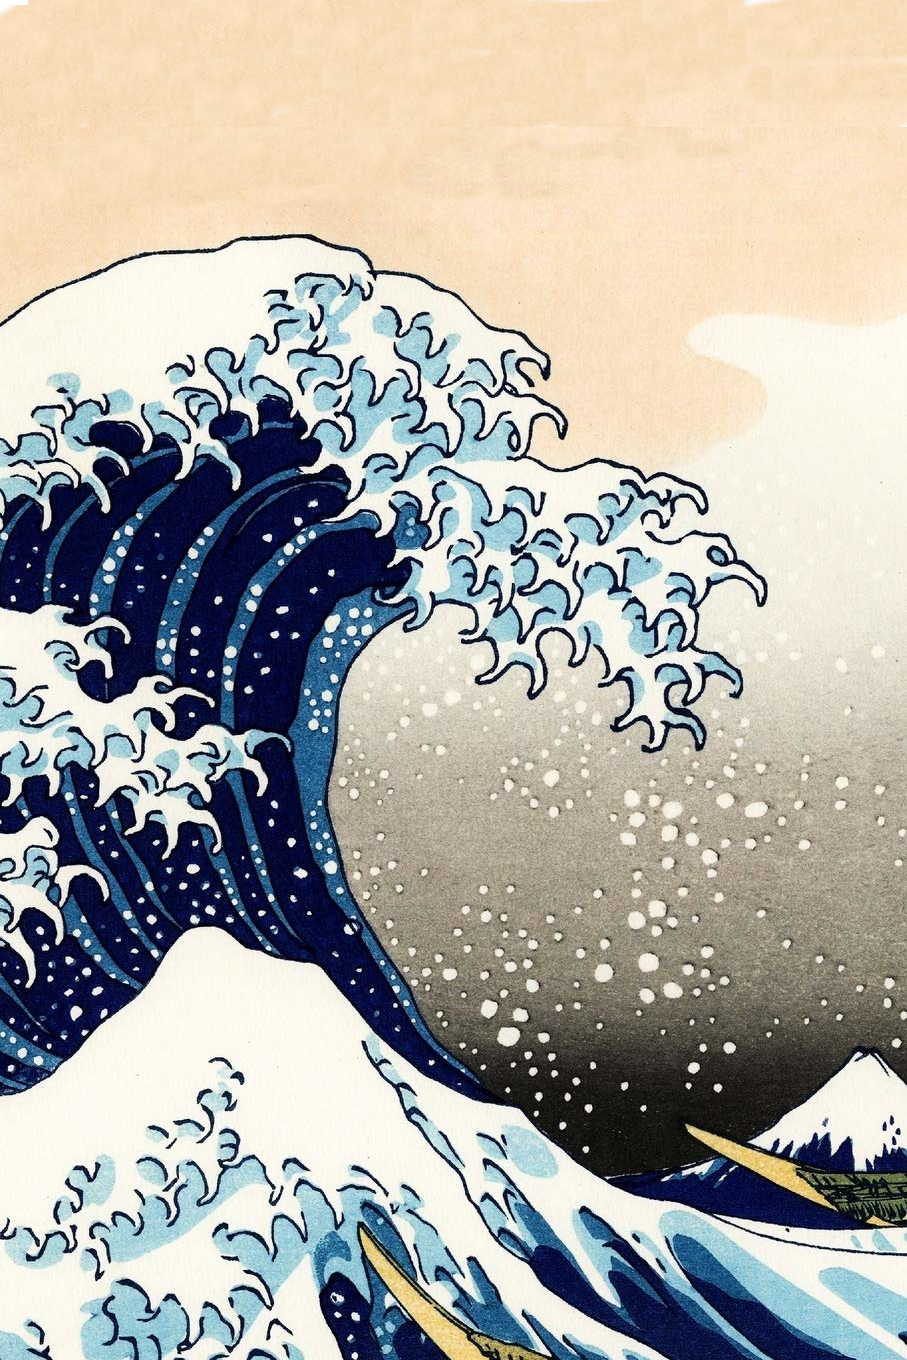
\includegraphics[width=\paperwidth,height=\paperheight]{img/covers/page.jpg}}%
}


%DIF LATEXDIFF DIFFERENCE FILE
%DIF DEL 03-etat-art.tex       Sun Apr  3 22:15:34 2022
%DIF ADD old-03-etat-art.tex   Thu Apr  7 00:23:48 2022
% !TeX spellcheck = fr_FR
%DIF PREAMBLE EXTENSION ADDED BY LATEXDIFF
%DIF UNDERLINE PREAMBLE %DIF PREAMBLE
\RequirePackage[normalem]{ulem} %DIF PREAMBLE
\RequirePackage{color}\definecolor{RED}{rgb}{1,0,0}\definecolor{BLUE}{rgb}{0,0,1} %DIF PREAMBLE
\providecommand{\DIFadd}[1]{{\protect\color{blue}\uwave{#1}}} %DIF PREAMBLE
\providecommand{\DIFdel}[1]{{\protect\color{red}\sout{#1}}}                      %DIF PREAMBLE
%DIF SAFE PREAMBLE %DIF PREAMBLE
\providecommand{\DIFaddbegin}{} %DIF PREAMBLE
\providecommand{\DIFaddend}{} %DIF PREAMBLE
\providecommand{\DIFdelbegin}{} %DIF PREAMBLE
\providecommand{\DIFdelend}{} %DIF PREAMBLE
%DIF FLOATSAFE PREAMBLE %DIF PREAMBLE
\providecommand{\DIFaddFL}[1]{\DIFadd{#1}} %DIF PREAMBLE
\providecommand{\DIFdelFL}[1]{\DIFdel{#1}} %DIF PREAMBLE
\providecommand{\DIFaddbeginFL}{} %DIF PREAMBLE
\providecommand{\DIFaddendFL}{} %DIF PREAMBLE
\providecommand{\DIFdelbeginFL}{} %DIF PREAMBLE
\providecommand{\DIFdelendFL}{} %DIF PREAMBLE
%DIF END PREAMBLE EXTENSION ADDED BY LATEXDIFF

\begin{document}
    \frontmatter

	\BgThispage
    \begin{titlepage}
            
\includegraphics[height=2cm]{img/covers/ubfc-logo}
            \hfill
            
\includegraphics[height=2cm]{img/covers/e2s-big}
            \vfill
            
            \begin{center}
	            \textbf{\bfseries THÈSE DE DOCTORAT DE L'UNIVERSITÉ \\ BOURGOGNE FRANCHE-COMTÉ \\ PRÉPARÉE À L'INRAE -- UMR AGROÉCOLOGIE} \\[1.5cm]
	        
	        	\textsc{École doctorale n°554, Environement-Santé} \\
	        	\textsc{Doctorat en Informatique} \\[.5cm]
	        	%\textsc{Par Jehan-Antoine Vayssade} \\[1cm]
	        	\textsc{Thèse présentée et soutenue par \\ \large Jehan-Antoine Vayssade \\ \small à Dijon le 08 mars 2022}\\[1.cm]
	        	
	        	{ \Large \bfseries Approche multi-critère \\ pour la caractérisation des adventices }
	        \end{center}
        	
            
            %\vfill
            %\textsc{\Large Thèse} \\[.5cm]
            %\textsc{Pour obtenir le grade de \\ Docteur en Informatique}\\[1.5cm]
            %{ \Large \bfseries Approche multi-critères \\ pour la caractérisation des adventices }\\[1.5cm]
            %\textsc{Présentée et soutenue par \\ \large Jehan-Antoine Vayssade \\ \small le \today}\\[1.5cm]
            
            \null \vfill
            \noindent
			\begin{tabularx}{\linewidth}{l}
				 \textbf{Composition du Jury :} \\[.25cm]
            \end{tabularx}
            \begin{tabularx}{\linewidth}{l X r l}
				 \textbf{Pr.} & \textbf{Christian Germain} 		& {Bordeaux Sciences Agro}      & Examinateur  \\
				 \textbf{Pr.} & \textbf{Bruno Tisseyre} 	    & {Institut Agro Montpellier}   & Rapporteur  \\
                 \textbf{Pr.} & \textbf{Laure Tougne-Rodet} 	& {Université Lumière - Lyon 2} & Rapporteure  \\
				 \textbf{Pr.} & \textbf{Christelle Gée} 		& {Institut Agro Dijon}         & Directrice de thèse \\
				 \textbf{Mc.} & \textbf{Jean-Noël Paoli} 		& {Institut Agro Dijon}         & Co-encadrant \\
				 \textbf{Mc.} & \textbf{Gawain Jones} 			& {Institut Agro Dijon}         & Co-encadrant \\
                 %\textbf{M.}  & \textbf{Thibault Cozic} 	    & {Entreprise SITIA}            & Invité \\
                 %\textbf{Dr.} & \textbf{Mathieu Bonneau} 	    & {INRAe -- URZ}                & Invité \\
			\end{tabularx}
    \end{titlepage}
	\newpage
	\thispagestyle{empty}
	\null \vfill
	\begin{framed}
		\noindent \textbf{Titre:} Approche multi-critère pour la caractérisation des adventices \\[1em]
		\noindent \textbf{Mots clés :}  Vision par ordinateur ; Analyse d'image ; Intelligence artificielle ; Statistiques ; Prédiction ; Agriculture de précision
		\begin{multicols}{2}
			\noindent \textbf{Résumé:} L'objectif de cette thèse est de mettre au point un moyen de détecter les adventices dans un champ à l'aide d'images multispectrales, afin de pouvoir déterminer quelles sont les adventices à éliminer pendant le cycle de culture en cours et plus particulièrement aux stades précoces. L'approche multi-critère s'intéresse à la disposition spatiale, à la signature spectrale, à la morphologie et à la texture des plantes présentes dans les parcelles. Ce manuscrit propose une méthode permettant de sélectionner les meilleurs critères pour une discrimination optimale dans un contexte donné. Préalablement à l'extraction de ces critères, un ensemble de méthodes ont été développées afin de corriger les erreurs du dispositif d'acquisition, de détecter précisément la végétation, puis d'identifier au sein de la végétation les individus sur lesquels les différents critères peuvent être extraits. Pour l'étape de détection des individus, il s'est révélé que l'échelle de la feuille était plus adaptée que celle de la plante. La détection de la végétation et l'identification des feuilles s'appuient sur des méthodes d'apprentissage profond, capables de traiter des feuillages denses. L'introduction de ces méthodes dans une chaîne de traitement usuelle constitue l'originalité de ce manuscrit où chaque partie a fait l'objet d'un article. Concernant le dispositif d'acquisition, une méthode de recalage des bandes spectrales a été développée, et les résultats montrent une précision de l'ordre du pixel. Ensuite, de nouveaux indices de végétation reposant sur de l'intelligence artificielle constituent l'une des avancées scientifiques de cette thèse. A titre indicatif, ces indices permettent d'atteindre 82.19\% de mIoU contre 63.93\%-73.71\% pour des indices standards et fonctionnent en environnement non-contrôlé. Par extension, une méthode de détection des feuilles a été définie. Elle repose sur la détection de leurs contours, et semble avantageuse sur nos données multispectrales. Finalement, les meilleurs couples de propriétés ont été définis pour la discrimination culture/adventices à l'échelle de la feuille, dont les performances atteignent 91\% de classification.
		\end{multicols}
	\end{framed}
	\vfill
	\newpage
    \thispagestyle{empty}
    \null
    \vfill
	\begin{framed}
		\noindent  \textbf{Title:} A multi-criteria approach to weed characterization \\[1em]
        \noindent \textbf{Keywords:}  Computer vision; Image analysis; Artificial intelligence; Statistics; Prediction; Precision agriculture
		\begin{multicols}{2}
			\noindent \textbf{Summary:} The objective of this thesis is to develop a way to detect weeds in a field using multispectral images, in order to determine which weeds should be eliminated during the current crop cycle and more particularly at the early stages. The multi-criteria approach focuses on the spatial arrangement, the spectral signature, the morphology and the texture of the plants located in the plots. This work proposes a method for selecting the best criteria for optimal discrimination for a given setup. Prior to the extraction of these criteria, a set of methods was developed in order to correct the errors of the acquisition device, to precisely detect the vegetation and then to identify within the vegetation the individuals on which the different criteria can be computed. For the individual detection step, it appears that leaf scale is more suitable than plant scale. Vegetation detection and leaf identification are based on deep learning methods capable of processing dense foliage. The introduction of these methods in a usual processing chain constitutes the originality of this manuscript where each part was the subject of an article. Concerning the acquisition device, a method of spectral band registration was developed. Then, new vegetation indices based on artificial intelligence constitute one of the scientific advances of this thesis. As an indication, these indices offer a mIoU of 82.19\% when standard indices ceil at 63.93\%-73.71\%. By extension, a leaf detection method was defined and is based on the detection of their contours, this method seems advantageous on our multispectral data. Finally, the best property pairs were defined for crop/weed discrimination at leaf level, whith classification performances up to 91\%.
		\end{multicols}
	\end{framed}
	\vfill
	
	\newpage
	\thispagestyle{empty}
	
	\subsection*{Contributions de l'auteur}
	
	\subsubsection*{Conférences}
	
	\begin{itemize}
		\item \textbf{Two-step multi-spectral registration via key-point detector and gradient similarity} February 2020 - Proceedings of the 15th International Joint Conference on Computer Vision, Imaging and Computer Graphics Theory and Applications : Valetta (Malta) - Jehan-Antoine Vayssade; Gawain Jones; Jean Noel Paoli; Christelle Gée
		\item \textbf{DeepIndices : Une nouvelle approche des indices de télédétection basée sur l'optimisation et l'approximation de fonctions par DeepLearning. Application aux indices de végétation sur des données non calibrées} July 2021 - RJCIA : Rencontres des Jeunes Chercheurs en Intelligence Artificielle (Bordeaux) - Jehan-Antoine Vayssade; Jean Noel Paoli; Christelle Gée; Gawain Jones
	\end{itemize}

	\subsubsection*{Articles de journaux internationaux}
	\begin{itemize}
		\item \textbf{DeepIndices: Remote Sensing Indices Based on Approximation of Functions through Deep-Learning, Application to Uncalibrated Vegetation Images} June 2021 - Remote Sensing 13(2261) - Jehan-Antoine Vayssade; Jean Noel Paoli; Christelle Gée; Gawain Jones
        \item \textbf{Dense Leaves Pixelwise Instance Segmentation} Febrary 2022 - Computer and Electronics in Agriculture - Jehan-Antoine Vayssade; Gawain Jones; Christelle Gée; Jean Noel Paoli
	\end{itemize}

	\subsubsection*{Article en cours de publication}
	\begin{itemize}
		\item \textbf{Weed discrimination at leaf scale: towards the characterization of the vegetation  cover} January 2022 - Computer and Electronics in Agriculture - Jehan-Antoine Vayssade, Gawain Jones, Christelle Gée and Jean-Noël Paoli
	\end{itemize}

	\subsubsection*{Collaborations extérieures}
	\begin{itemize}
		\item \textbf{Automatic activity tracking of goats using drone camera} July 2019 - Computers and Electronics in Agriculture 162:767-772 - Jehan-Antoine Vayssade; Rémy Arquet; Mathieu Bonneau
		\item \textbf{Goats monitoring at the pasture scale combining neural network and time-lapse cameras} August 2019 - European Conference on Precisions Livestock Farming (ECPLF), - Mathieu Bonneau; Jehan-Antoine Vayssade; Willy Troupe; Rémy Arquet
		\item \textbf{Outdoor animal tracking combining neural network and time-lapse cameras} December 2019 - Computers and Electronics in Agriculture 168 - Mathieu Bonneau; Jehan-Antoine Vayssade; Willy Troupe; Rémy Arquet
	\end{itemize}

	%\subsection*{Base de données ouvertes}
	%\begin{itemize}
	%	\item \textbf{Dataset used in DeepIndices} - 2021/05/26 - doi: 10.15454/DSQC8N - Jehan-Antoine Vayssade
	%	\item \textbf{Multi-Spectral Leaf Segmentation For Crop / Weed Identification} - 2021/06/24 - doi: 10.15454/JMKP9S- Jehan-Antoine Vayssade
	%\end{itemize}

	\null
	\newpage

    %\cleardoublepage
    %\thispagestyle{empty}
    %{\noindent%
    %    \huge{\textbf{\textsf{Declaration of Authorship}}}
    %}
    %\vspace{2cm}
    %\begin{flushleft}
    %    \noindent%
    %    I declare that the work presented here is original and the result of my own investigations.
    %    Formulations and ideas taken from other sources are cited as such.
    %
    %    It has not been submitted, either in part or whole, for a degree at this or any other university.
    %\end{flushleft}
    %
    %\vspace{8cm}
    %\noindent%
    %\rule[1em]{8em}{0.5pt}  \hfill \rule[1em]{8em}{0.5pt}\\ % This prints a line to write the date
    %Location, Date \hfill Signature\\
    %\cleardoublepage
    
    \mainmatter
    %\subfile{content/00-remerciement}
    \subfile{content/01-preambule.tex}
    \thispagestyle{empty}
    \tableofcontents
    
    %\addtocontents{toc}{\protect\vspace{-2em}}
    \subfile{content/02-introduction.tex} % .diff
    \addtocontents{toc}{\protect\thispagestyle{empty}}
    \subfile{content/03-etat-art.tex} % .diff
    
    %\addtocontents{toc}{\protect\newpage}
    %\addtocontents{toc}{\protect\thispagestyle{empty}}
    \subfile{content/04-material-and-data.tex} % .diff
    %\subfile{content/05-preprocessing.tex} %.diff
    \subfile{content/05-article}
    \subfile{content/06-vegetation-indices.tex} % .diff
    \addtocontents{toc}{\protect\newpage}
    \addtocontents{toc}{\protect\thispagestyle{empty}}
    \subfile{content/07-detection-feuille.tex} % .diff
    \subfile{content/08-leaf-features.tex} % .diff
    \subfile{content/09-conclusion.tex} % .diff
	\listoffigures
	\listoftables

	\bibliography{thesis.bib}
	\bibliographystyle{apalike}

\end{document}

